\documentclass{beamer}
\usepackage{beamerthemesplit}
\usepackage{wrapfig}
\usetheme{SPbGU}
\usepackage{pdfpages}
\usepackage{amsmath}
\usepackage{cmap} 
\usepackage[T2A]{fontenc} 
\usepackage[utf8]{inputenc}
\usepackage[english,russian]{babel}
\usepackage{indentfirst}
\usepackage{amsmath}
\usepackage{tikz}
\usepackage{multirow}
\usepackage[noend]{algpseudocode}
\usepackage{algorithm}
\usepackage{algorithmicx}
\usetikzlibrary{shapes,arrows}
\usepackage{fancyvrb}

\usepackage{graphicx}
\usepackage[utf8]{inputenc}  
\usepackage{amsmath}
\usepackage{amssymb}
\usepackage{amsthm}
\usepackage{latexsym}
\usepackage{float}
\usepackage{tabularx}
\usepackage{booktabs}

\allowdisplaybreaks

\newtheorem{rutheorem}{Теорема}
\newtheorem{ruproof}{Доказательство}
\newtheorem{rudefinition}{Определение}
\newtheorem{rulemma}{Лемма}

\beamertemplatenavigationsymbolsempty

\title[]{Парсер-комбинаторы и Parser Expression Grammars}
\subtitle[]{}
% То, что в квадратных скобках, отображается в левом нижнем углу. 
\institute[]{
Санкт-Петербургский государственный университет \\
Математико-механический факультет }

% То, что в квадратных скобках, отображается в левом нижнем углу.
\author[Екатерина Вербицкая]{Екатерина Вербицкая}

\date{8 декабря 2015г.}

\definecolor{orange}{RGB}{179,36,31}

\begin{document}
{
\begin{frame}[fragile]
  \titlepage
\end{frame}
}

\begin{frame}[fragile]
  \transwipe[direction=90]
  \frametitle{Долг: зачем нужен RNGLR}
\pause 
Для обработки неоднозначных грамматик. Часто нельзя выбрать заранее, какая из альтернатив "верна".

\pause

$$
\begin{array}{crcl}
&S & \rightarrow & if \, b \, then \, S \, else \, S \\ 
&S & \rightarrow & if \, b \, then \, S \\ 
&S & \rightarrow & a \\ 
\end{array}
$$   	            

\pause 
2 дерева вывода для цепочки $if \, b \, then \, if \, b \, then \, a \, else \, a$             


\end{frame}


\begin{frame}[fragile]
  \transwipe[direction=90]
  \frametitle{Лес разбора: объединяет 2 дерева}
\begin{center}
  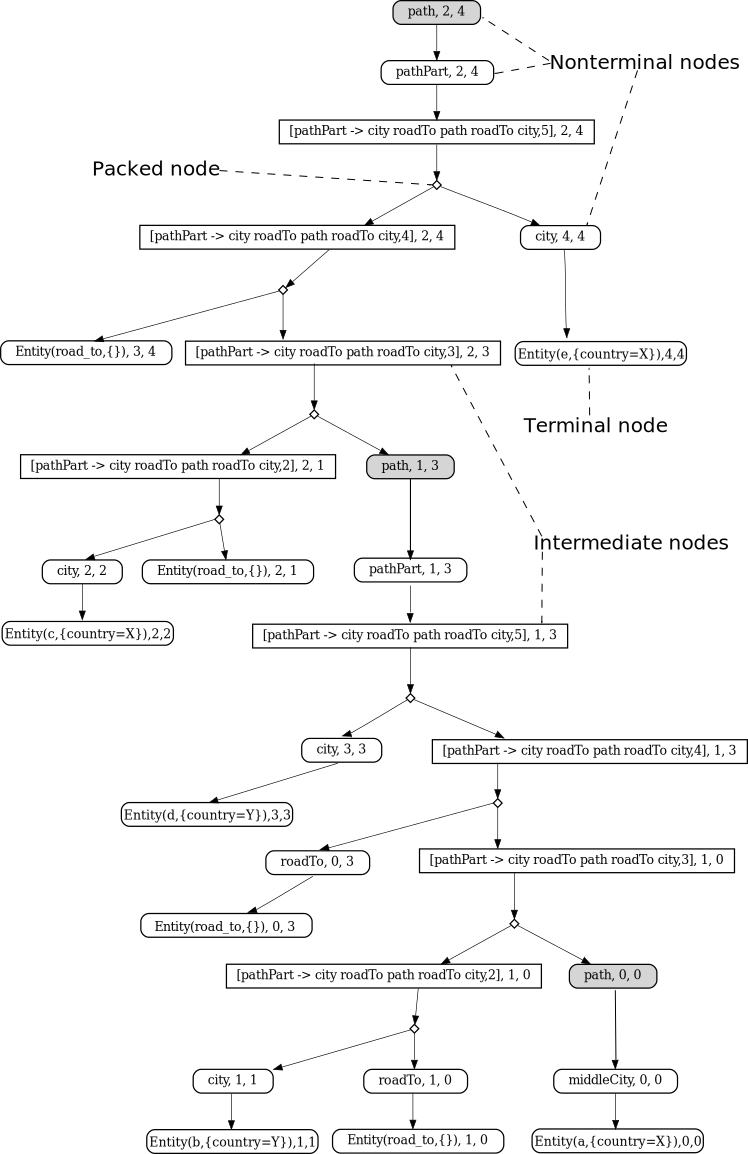
\includegraphics[width=0.8\textwidth]{pics/sppf} 
\end{center}
\end{frame}




\begin{frame}[fragile]
  \transwipe[direction=90]
  \frametitle{Парсер-комбинаторы: общая идея}
  \begin{itemize}
    \item Написать примитивные парсеры (например, для обработки отдельных 
символов)
    \item Написать комбинаторы для составления из примитивных парсеров более 
сложных
    \begin{itemize}
      \item Последовательности
      \item Альтернативы
      \item Повторение
      \item Опциональный парсер
      \item \dots
    \end{itemize}
    \item С использованием этого инструментария описать необходимый парсер
  \end{itemize}
\end{frame}

\begin{frame}
  \transwipe[direction=90]
  \frametitle{Парсер-комбинаторы: тип парсера}
$$
\begin{array}{crcl}
&Parser & = & String \rightarrow Tree \\ \pause
&Parser & = & String \rightarrow (Tree, String) \\ \pause
&Parser & = & String \rightarrow [(Tree, String)] \\ \\ \pause
&Parser \, a & = & String \rightarrow [(a, String)]
\end{array}
$$
\end{frame}

\begin{frame}[fragile]
  \transwipe[direction=90]
  \frametitle{Примитивные парсеры}
\begin{verbatim}
result :: a -> Parser a
result v = \inp -> [(v,inp)]

zero :: Parser a
zero = \inp -> []

item :: Parser Char
item = \inp -> case inp of
                 [] -> []
                 (x:xs) -> [(x,xs)]
\end{verbatim}  
\end{frame}

\begin{frame}[fragile]
  \transwipe[direction=90]
  \frametitle{Парсер-комбинаторы}
\begin{verbatim}
bind :: Parser a -> (a -> Parser b) -> Parser b
p ‘bind‘ f = \inp -> concat [f v inp' | (v,inp') <- p inp]

p ‘seq‘ q = p ‘bind‘ \x ->
            q ‘bind‘ \y ->
            result (x,y)

sat :: (Char -> Bool) -> Parser Char
sat p = item ‘bind‘ \x ->
        if p x then result x else zero

plus :: Parser a -> Parser a -> Parser a
p ‘plus‘ q = \inp -> (p inp ++ q inp)
\end{verbatim}
\end{frame}

\begin{frame}[fragile]
  \transwipe[direction=90]
  \frametitle{Маленькие полезные парсеры}
\begin{verbatim}
char :: Char -> Parser Char
char x = sat (\y -> x == y)

digit :: Parser Char
digit = sat (\x -> ’0’ <= x && x <= ’9’)

lower :: Parser Char
lower = sat (\x -> ’a’ <= x && x <= ’z’)

upper :: Parser Char
upper = sat (\x -> ’A’ <= x && x <= ’Z’)
\end{verbatim}
\end{frame}

\begin{frame}[fragile]
  \transwipe[direction=90]
  \frametitle{Менее маленькие полезные парсеры}
\begin{verbatim}
letter :: Parser Char
letter = lower ‘plus‘ upper

alphanum :: Parser Char
alphanum = letter ‘plus‘ digit

word :: Parser String
word = neWord ‘plus‘ result ""
       where
         neWord = letter ‘bind‘ \x ->
                  word ‘bind‘ \xs ->
                  result (x:xs)

word "Yes!" = [("Yes","!"), ("Ye","s!"), 
               ("Y","es!"), ("","Yes!")]
\end{verbatim}
\end{frame}

\begin{frame}[fragile]
  \transwipe[direction=90]
  \frametitle{Монадические парсер-комбинаторы}
\begin{verbatim}
class Monad m where
  result :: a -> m a
  bind :: m a -> (a -> m b) -> m b

instance Monad Parser where
  -- result :: a -> Parser a
  result v = \inp -> [(v,inp)]

  -- bind :: Parser a -> (a -> Parser b) -> Parser b
  p ‘bind‘ f = \inp -> concat [f v out | (v,out) <- p inp]
\end{verbatim}
\end{frame}

\begin{frame}[fragile]
  \transwipe[direction=90]
  \frametitle{Монадические парсер-комбинаторы}
\begin{verbatim}
class Monad m => Monad0Plus m where
  zero :: m a
  (++) :: m a -> m a -> m a

instance Monad0Plus Parser where
  -- zero :: Parser a
  zero = \inp -> []
  
  -- (++) :: Parser a -> Parser a -> Parser a
  p ++ q = \inp -> (p inp ++ q inp)
\end{verbatim}
\end{frame}

\begin{frame}[fragile]
  \transwipe[direction=90]
  \frametitle{Другая форма записи}
\begin{verbatim}
p1 ‘bind‘ \x1 ->
p2 ‘bind‘ \x2 ->
...
pn ‘bind‘ \xn ->
result (f x1 x2 ... xn)


[ f x1 x2 ... xn | x1 <- p1
                 , x2 <- p2
                 , ...
                 , xn <- pn ]

string :: String -> Parser String
string "" = [""]
string (x:xs) = [x:xs | _ <- char x, _ <- string xs]
\end{verbatim}
\end{frame}

\begin{frame}[fragile]
  \transwipe[direction=90]
  \frametitle{Монадические парсер-комбинаторы}
\begin{verbatim}
sat :: (Char -> Bool) -> Parser Char
sat p = [x | x <- item, p x]

many :: Parser a -> Parser [a]
many p = [x:xs | x <- p, xs <- many p] ++ [[]]



ident :: Parser String
ident = [x:xs | x <- lower, xs <- many alphanum]
\end{verbatim}
\end{frame}

\begin{frame}[fragile]
  \transwipe[direction=90]
  \frametitle{Примеры парсеров}
\begin{verbatim}
many1 :: Parser a -> Parser [a]
many1 p = [x:xs | x <- p, xs <- many p]

nat :: Parser Int
nat = [eval xs | xs <- many1 digit]
      where
        eval xs = foldl1 op [ord x - ord ’0’ | x <- xs]
        m ‘op‘ n = 10*m + n

int :: Parser Int
int = [-n | _ <- char ’-’, n <- nat] ++ nat

int :: Parser Int
int = [f n | f <- op, n <- nat]
      where
        op = [negate | _ <- char ’-’] ++ [id]
\end{verbatim}
\end{frame}


\begin{frame}[fragile]
  \transwipe[direction=90]
  \frametitle{Пример: список чисел}
\begin{verbatim}
ints :: Parser [Int]
ints = [n:ns | _ <- char ’[’
             , n <- int
             , ns <- many [x | _ <- char ’,’, x <- int]
             , _ <- char ’]’]


sepby1 :: Parser a -> Parser b -> Parser [a]
p ‘sepby1‘ sep = [x:xs | x <- p
                       , xs <- many [y | _ <- sep, y <- p]]

ints = [ns | _ <- char ’[’
           , ns <- int ‘sepby1‘ char ’,’
           , _ <- char ’]’]

\end{verbatim}
\end{frame}


\begin{frame}[fragile]
  \transwipe[direction=90]
  \frametitle{Список чисел: еще короче}
\begin{verbatim}
bracket :: Parser a -> Parser b -> Parser c -> Parser b
bracket open p close = [x | _ <- open, x <- p, _ <- close]

ints = bracket (char ’[’)
               (int ‘sepby1‘ char ’,’)
               (char ’]’)
\end{verbatim}
\end{frame}


\begin{frame}[fragile]
  \transwipe[direction=90]
  \frametitle{Пример: арифметические выражения}
$$
\begin{array}{crcl}
&expr & ::= & expr \, addop \, factor \, | \, factor \\ 
&addop & ::= & + \, | \, - \\ 
&factor & ::= & nat \, | \, ( \, expr \, ) \\
\end{array}
$$ 

\begin{verbatim}

expr :: Parser Int
addop :: Parser (Int -> Int -> Int)
factor :: Parser Int

expr = [f x y | x <- expr
              , f <- addop
              , y <- factor] ++ factor

addop = [(+) | _ <- char ’+’] ++ [(-) | _ <- char ’-’]

factor = nat ++ bracket (char ’(’) expr (char ’)’)
\end{verbatim}
\end{frame}

\begin{frame}[fragile]
  \transwipe[direction=90]
  \frametitle{Избавляемся от левой рекурсии}

\begin{verbatim}
expr = [foldl (\x (f,y) -> f x y) x fys
           | x <- factor
           , fys <- many [(f,y) | f <- addop, y <- factor]]

addop = [(+) | _ <- char ’+’] ++ [(-) | _ <- char ’-’]

factor = nat ++ bracket (char ’(’) expr (char ’)’)
\end{verbatim}
\end{frame}

\begin{frame}[fragile]
  \transwipe[direction=90]
  \frametitle{Преимущества монадических парсер-комбинаторов}
  \begin{itemize}
    \item Простота
    \item Гибкость
    \item Выразительность
    \item Возможность откатываться (backtracking)
    \item Лексический анализ не нужно выделять в отдельный шаг
    \item Можно считать семантику во время синтаксического анализа
  \end{itemize}
\end{frame}

\begin{frame}[fragile]
  \transwipe[direction=90]
  \frametitle{Недостатки монадических парсер-комбинаторов}
  \begin{itemize}
    \item Если использовать неграмотно, можно получить непредсказуемое время 
работы и легко исчерпать всю доступную память
    \begin{itemize}
      \item Наличие общих префиксов у нескольких правил. Решение: факторизация грамматики
      \item Вычисление промежуточных результатов, где не было надо. Решение: использование ленивости (например, $p +++ q = first (p ++ q)$)
    \end{itemize}
  \end{itemize}
\end{frame}


\begin{frame}[fragile]
  \transwipe[direction=90]
  \frametitle{Parser Expression Grammars}
\begin{itemize}
  \item PEG G --- четверка $(V, T, P, p_S)$, где 
    \begin{itemize}
      \item $V$ --- конечное множество нетерминалов
      \item $T$ --- алфавит (конечное множество терминалов) 
      \item $P$ --- функция из $V$ в выражения (parser expression) 
      \item $p_S$ --- стартовое выражение
    \end{itemize}
\end{itemize}
\begin{itemize}
  \item Parser expression
  \begin{itemize}
    \item Пустая строка $\varepsilon$
    \item Терминал $a$
    \item Нетерминал $A$
    \item Последовательность $p_1 p_2$, где $p_1, p_2$ --- parser expression
    \item Упорядоченный выбор $p_1 / p_2$, где $p_1, p_2$ --- parser expression
    \item 0-или-больше $p^*$, где $p$ --- parser expression
    \item Предикат Не $!p$, где $p$ --- parser expression
  \end{itemize}
\end{itemize}
\end{frame}

\begin{frame}[fragile]
  \transwipe[direction=90]
  \frametitle{Отношение PEG}
\begin{center}
  \includegraphics[width=0.3\textwidth]{pics/pegRel}
\end{center}                                      
\begin{itemize}
  \item Выражение \textit{p} парсит строку \textit{xy}, съедая \textit{x} и оставляя \textit{y}, возвращая 
\textit{x'} как результат
  \item Если справа \textit{fail}, значит, распарсить строку не удалось
\end{itemize}
\end{frame}

\begin{frame}[fragile]
  \transwipe[direction=90]
  \frametitle{Операционная семантика PEG: пустая строка}
\begin{center}
  \includegraphics[width=0.3\textwidth]{pics/empty}
\end{center}                                      
\end{frame}

\begin{frame}[fragile]
  \transwipe[direction=90]
  \frametitle{Операционная семантика PEG: терминал}
\begin{center}
  \includegraphics[width=0.35\textwidth]{pics/char1}  \\~\\   \pause
  \includegraphics[width=0.5\textwidth]{pics/char2}   \\~\\   \pause
  \includegraphics[width=0.3\textwidth]{pics/char3}
\end{center}  
\end{frame}

\begin{frame}[fragile]
  \transwipe[direction=90]
  \frametitle{Операционная семантика PEG: переменная}
\begin{center}
  \includegraphics[width=0.4\textwidth]{pics/var1}  \\~\\     \pause
  \includegraphics[width=0.35\textwidth]{pics/var2} 
\end{center}
\end{frame}


\begin{frame}[fragile]
  \transwipe[direction=90]
  \frametitle{Операционная семантика PEG: последовательность}
\begin{center}
  \includegraphics[width=0.7\textwidth]{pics/con1}  \\~\\     \pause
  \includegraphics[width=0.7\textwidth]{pics/con2}  \\~\\     \pause
  \includegraphics[width=0.35\textwidth]{pics/con3}
\end{center}
\end{frame}

\begin{frame}[fragile]
  \transwipe[direction=90]
  \frametitle{Операционная семантика PEG: выбор}
\begin{center}
  \includegraphics[width=0.4\textwidth]{pics/ord1}  \\~\\     \pause
  \includegraphics[width=0.6\textwidth]{pics/ord2}  \\~\\     \pause
  \includegraphics[width=0.65\textwidth]{pics/ord3}
\end{center}
\end{frame}

\begin{frame}[fragile]
  \transwipe[direction=90]
  \frametitle{Операционная семантика PEG: предикат не}
\begin{center}
  \includegraphics[width=0.3\textwidth]{pics/not1}  \\~\\     \pause
  \includegraphics[width=0.35\textwidth]{pics/not2} 
\end{center}
\end{frame}

\begin{frame}[fragile]
  \transwipe[direction=90]
  \frametitle{Операционная семантика PEG: повторение}
\begin{center}
  \includegraphics[width=0.3\textwidth]{pics/rep1}  \\~\\     \pause
  \includegraphics[width=0.7\textwidth]{pics/rep2} 
\end{center}
\end{frame}

\begin{frame}[fragile]
  \transwipe[direction=90]
  \frametitle{Борьба с левой рекурсией: ограниченная левая рекурсия}
\begin{itemize}
  \item $A^n$ имеет не более $n$ леворекурсивных вызовов $A$, $A^0$ всегда 
завершается ошибкой
\end{itemize}
$$
\begin{array}{crcl}
&E^0 & ::= & fail \\ 
&E^1 & ::= & E^0 + n / n = \bot + n / n = n \\
&E^2 & ::= & E^1 + n / n = n + n / n \\
&E^3 & ::= & E^2 + n / n = (n + n / n) + n / n\\
& & \dots &  \\
&E^n & ::= & E^{n-1} + n / n \\
\end{array}
$$ 
\end{frame}


\begin{frame}[fragile]
  \transwipe[direction=90]
  \frametitle{Пример: разбираем с разными границами строку $n \, + \, n$}
$$
\begin{array}{crcl}
&E^0 (n \, + \, n) & = & fail \\ 
&E^1 (n \, + \, n) & = & (\bot + n / n) (n  +  n) = (n, +  n) \\
&E^2 (n \, + \, n) & = & (n + n / n) (n + n) = (n + n, \varepsilon) \\~\\
&E^3 (n \, + \, n) & = & ((n + n / n) + n / n) (n + n) = (n, + n) \\
\end{array}
$$ 

При разборе входа с помощью $E^3$, во внутренней альтернативе $(n + n / n)$ 
первый вариант срабатывает (и поэтому второй вариант не будет рассматриваться вообще!). 
После этого пытаемся разобрать оставшийся $\varepsilon$ с помощью оставшегося $+ n$ и не можем. 
Остается только вторая альтернатива, поэтому матчится только один $n$.
\end{frame}


\begin{frame}[fragile]
  \transwipe[direction=90]
  \frametitle{Борьба с левой рекурсией}
\begin{itemize}
  \item Ищем значение $n$ для каждого леворекурсивного нетерминала
  \item Подбирается такая граница, чтобы префикс, обработанный правилом, имел 
максимальную длину
  \item Промежуточные значения сохраняются в табличку $L$
  \begin{itemize}
    \item $L[(A, x) \rightarrow X](B, y) = L(B, y)$, если $B \neq A$ или $y 
\neq x$
    \item $L[(A, x) \rightarrow X](A, x) = X$
  \end{itemize}
\end{itemize}
\end{frame}

\begin{frame}[fragile]
  \transwipe[direction=90]
  \frametitle{Обработка леворекурсивного нетерминала}
\begin{center}
  \includegraphics[width=1.0\textwidth]{pics/lvar1}  \\~\\     \pause
  \includegraphics[width=0.7\textwidth]{pics/lvar2}  \\~\\     \pause 
  \includegraphics[width=0.3\textwidth]{pics/lvar3}  \\~\\     \pause
  \includegraphics[width=0.35\textwidth]{pics/lvar4}  
\end{center}
\end{frame}

\begin{frame}[fragile]
  \transwipe[direction=90]
  \frametitle{Семантика отношения INC}
\begin{center}
  \includegraphics[width=1.0\textwidth]{pics/incr1}  \\~\\     \pause
  \includegraphics[width=0.3\textwidth]{pics/incr2}  \\~\\     \pause
  \includegraphics[width=0.7\textwidth]{pics/incr3}  
\end{center}
\end{frame}



\begin{frame}[fragile]
  \transwipe[direction=90]
  \frametitle{Литература}
\begin{itemize}
  \item Monadic parser combinators: \url{http://www.cs.nott.ac.uk/~pszgmh/monparsing.pdf}
  \item Left recursion in Parsing Expression Grammars: \url{http://arxiv.org/pdf/1207.0443.pdf}
  \item Парсер-комбинаторная библиотека на F\#: \url{https://github.com/pragmatrix/ScanRat}
\end{itemize}

\end{frame}
\end{document}
